% Created 2020-01-29 Wed 13:00
% Intended LaTeX compiler: pdflatex
\documentclass[a4paper, justified, notitlepage, sfsidenotes, notoc]{tufte-book}
     \input{/users/rakhim/.emacs.d/latex/tufte.tex}
\usepackage[utf8]{inputenc}
\usepackage[T1]{fontenc}
\usepackage{graphicx}
\usepackage{grffile}
\usepackage{longtable}
\usepackage{wrapfig}
\usepackage{rotating}
\usepackage[normalem]{ulem}
\usepackage{amsmath}
\usepackage{textcomp}
\usepackage{amssymb}
\usepackage{capt-of}
\usepackage{hyperref}
\date{}
\title{Computer Science For The Busy Developer}
\hypersetup{
 pdfauthor={Rakhim Davletkaliyev},
 pdftitle={Computer Science For The Busy Developer},
 pdfkeywords={},
 pdfsubject={},
 pdfcreator={Emacs 26.3 (Org mode 9.1.9)},
 pdflang={English}}
\begin{document}

\part{Intro to complexity}
\label{sec:org40a2477}

The proper way to discuss computational complexity would probably look like this: start with the idea of computation, describe models of computation (e.g. Turing machines and/or Lambda calculus), discuss limits of computation, explore automatons and languages (not programming languages, but formal languages derived from formal grammars like Context-free grammar), and then, finally, discuss the ways we can count the number of operations for certain algorithms.

Since this isn't an academic textbook (and we're busy developers), we will talk about computational complexity from the points of view of everyday programming. Nevertheless, the computability of the Universe, models of computations and their limits are very interesting and important (in that order!) topics. A separate chapter will focus on those.

You probably have at least a vague idea about algorithms. Often, analogies are used:

\begin{itemize}
\item meal recipe
\item walking instructions
\item emergency situation instructions
\end{itemize}

It's important to distinguish between the general idea of algorithm and the precise, formal, mathematical algorithms used in computer science. The ones above are \emph{examples} of regular, every-day algorithms. They aren't really analogies, but we don't think of them as algorithms, simply because they are too vague, open to interpretation. "Fry onions on medium heat until brown" — how brown is brown enough? what is medium heat? what exact light frequencies and temperatures are we talking about?!

The reason such instructions aren't extremely precise is that for the most part they're enough. The recipes are more like suggestions. People can make their own decisions and interpretations.

But computers can't. Computers can only follow precise, unambiguous instructions. Yet, the roots of this formal nature of algorithms are much older than digital computers. The word "algorithm" itself was derived from the name of Muhammad ibn Musa al-Khwarizmi, a Persian scholar who lived between in years 780-850. His books described algorithms for calculating certain numbers. These algorithms — instructions — must be precise and unambiguous even though they were created for mortal humans.



\begin{marginfigure}
  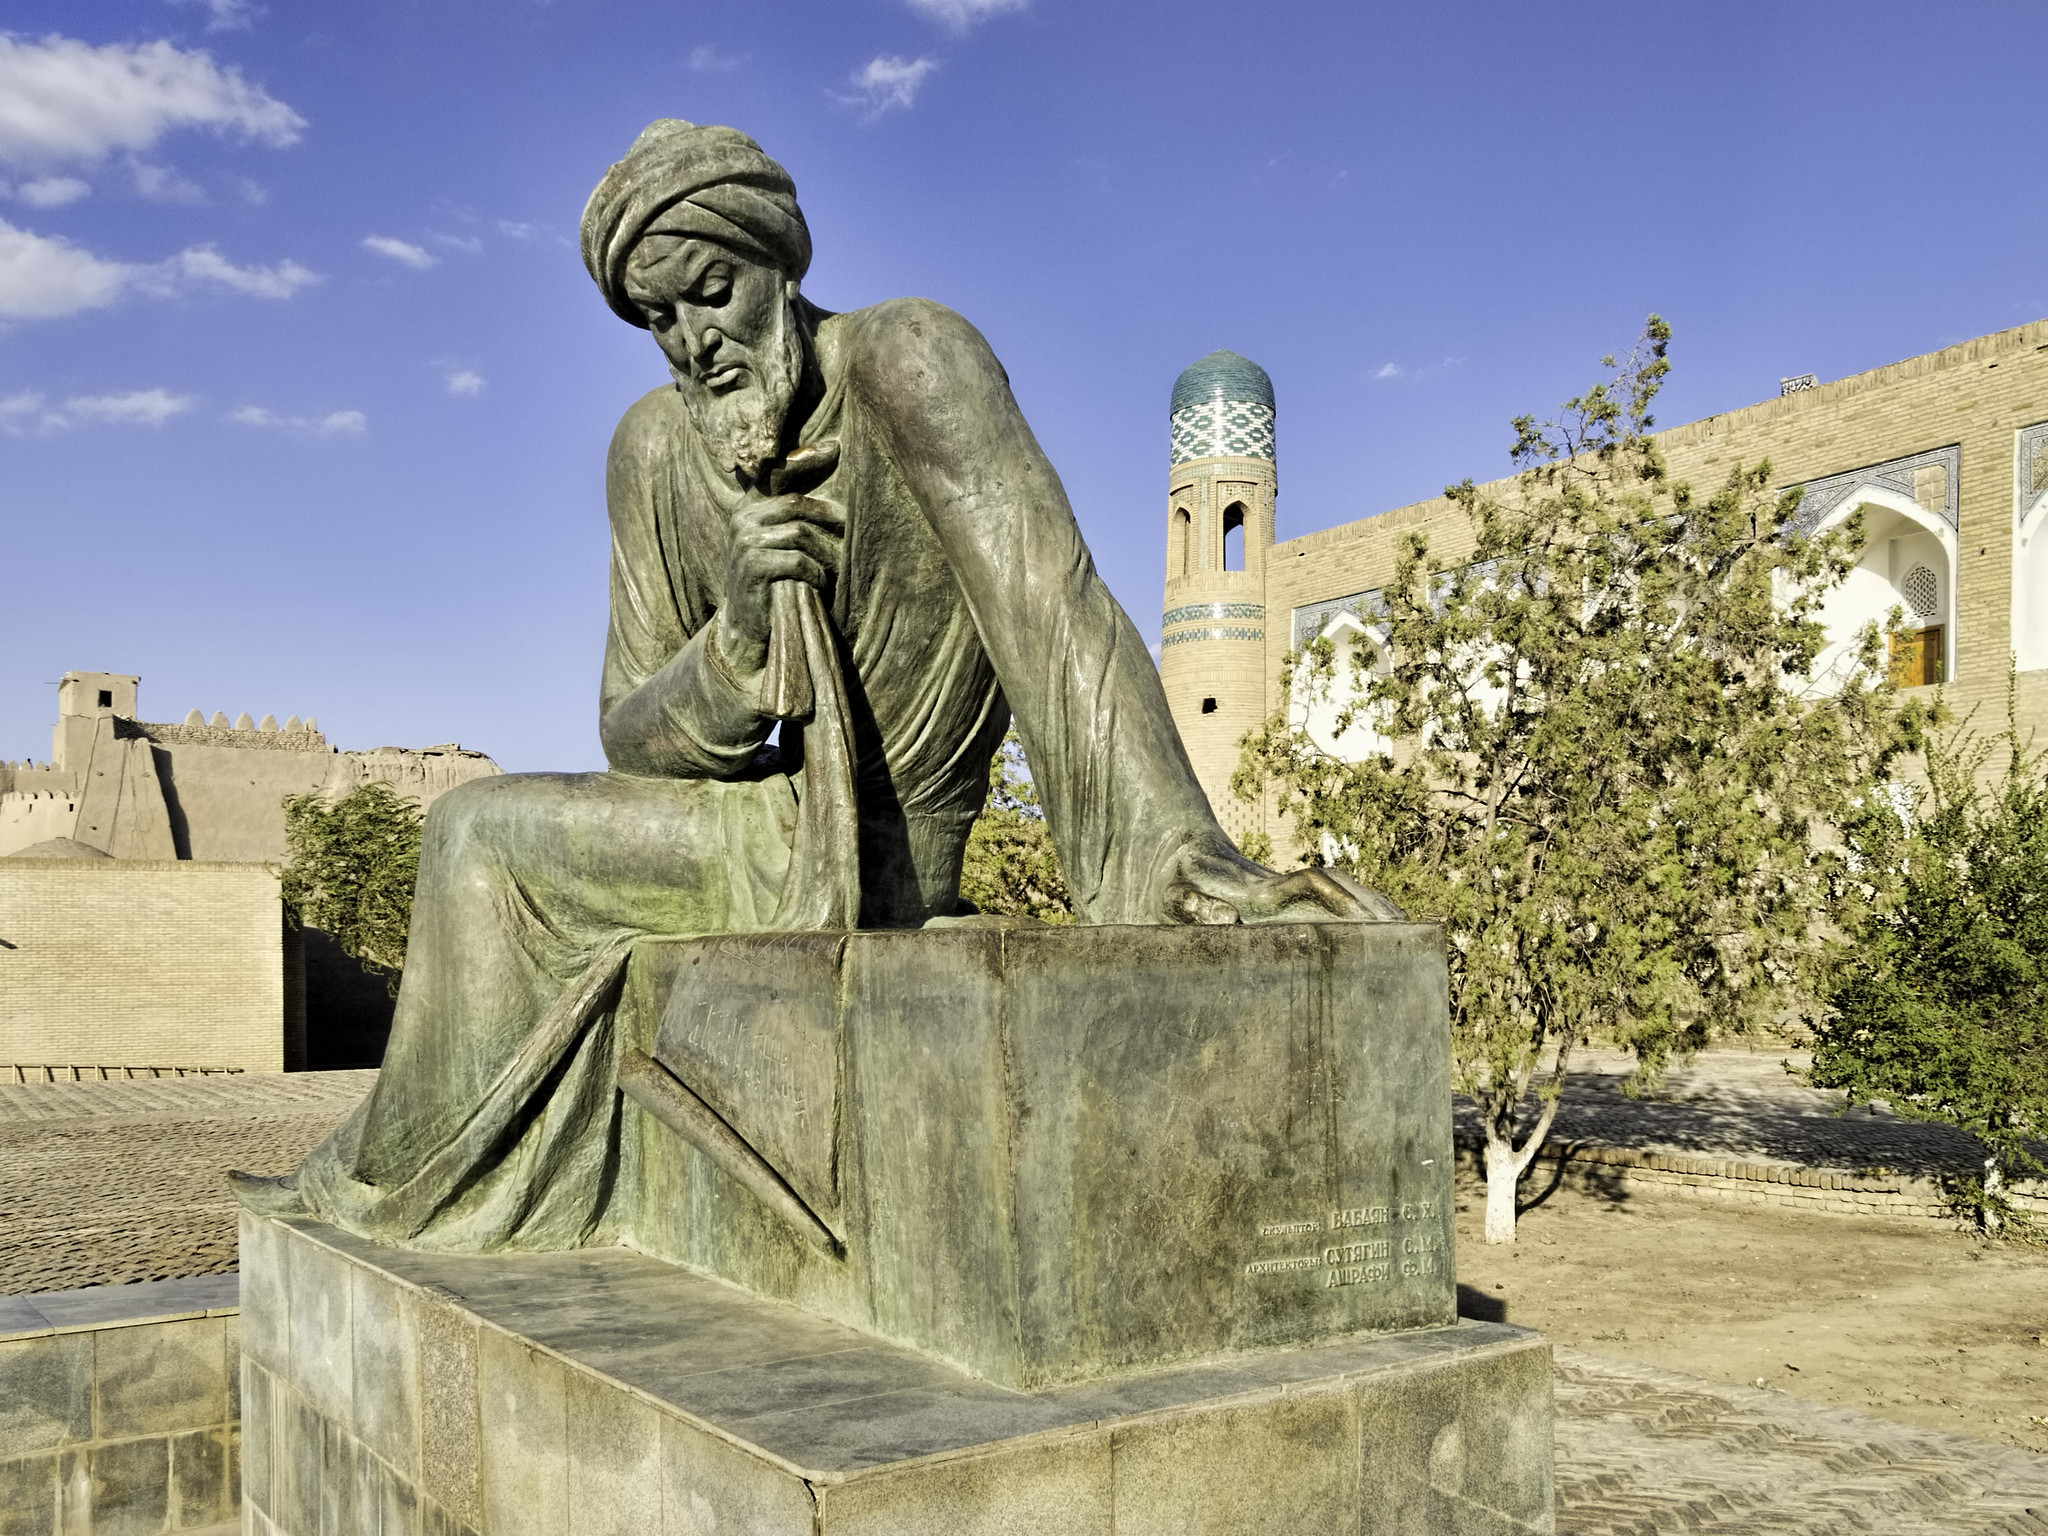
\includegraphics[width=\linewidth]{images/Muhammad ibn Musa al-Khwarizmi.jpg}
  \caption{Statue of Muhammad ibn Musa al-Khwarizmi, just outside Khiva’s west wall, Uzbekistan. Photo by Dan Lundberg.}
  \label{fig:marginfig}
\end{marginfigure}
\end{document}
